\section{Experiments}
\label{sec:experiments}

\subsection{The influence of synthesized segmention noises on feature transferability}
\label{subsec:robustness}

%%%%%%%% TEXT Experiment setup

\paragraph{Experiment setup}

To investigate the influence of inexhaustive segmentations, misclassifications and false segmentations on feature transferability, we set up experiments with synthesized label noises from a well-annotated dataset, the PASCAL VOC2011 segmentation dataset  \cite{everingham2015pascal}.
Fifteen out of twenty categories of the VOC2011 dataset were selected to form a \textit{pre-training dataset} and the other categories formed a \textit{fine-tuning dataset}.
The pre-training dataset was used to train a Fully Convolutional Network with AlexNet (FCN-AlexNet) model \cite{long2015fully} for segmentation in the presence or absence of synthesized segmentation errors.
The fine-tuning dataset was used to fine-tune the weights of convolutional layers from the pre-trained FCN-AlexNet models.
Inexhaustive segmentations, misclassifications, and false segmentations were synthesized separately with stochastical corruptions to the well-annotated pre-training dataset, followed the descriptions in Section \ref{subsec:formulation}.
Fine-tuned models were evaluated by mean intersection over union ratio (mean IU) achieved on the fine-tuning test set, referring to as the \textit{fine-tuning performance}.
Performance improvement of fine-tuning transferred models compared to an randomly initialized model indicates the transferability of pre-trained weights.

\paragraph{Experiment details}

To avoid that the choice of pre-training and fine-tuning splitting for categories influence the results, the 20 categories of VOC2011 were divided equally into four folds.
Each fold was studied separately, and the exact partitions of each fold are listed in Table \ref{tab:robustness}.
The training dataset was enriched with extra segmentations by Hariharan et al. \cite{hariharan2011semantic}
To keep the segmentation task simple, we used only single-object images, resulting in totally 4000 training images for 20 categories available for pre-training, fine-tuning and evaluation.
In order to accelerate the training process, we subsampled the original images by four times.
Fully Convolutional Networks with AlexNet was used for experiments because of its relatively small capacity and thus short training time.
The existence of an ImageNet model for AlexNet can be beneficial to set a performance reference.
The non-transferred layers were randomly initialized with Xavier Initialization.
The ImageNet model and completely random weight initialization were considered as the upper bound and lower bound, respectively, for various pre-trained weights summarized in Table \ref{tab:robustness}.
The default hyperparameters of FCN-AlexNet in  \cite{long2015fully} were kept unchanged.
Training run 240,000 iterations for pre-training phase, and 12,000 iterations for fine-tuning phase.
Snapshots for trained models were taken every 4,000 iterations.
Each experiment was repeated three times, mean and standard deviation were computed over the last five snapshots for all repetitions.


% \noindent \textit{What Table \ref{tab:robustness} tell us.
% How annotation errors were synthesized;
% How synthesizations are different from reality;
% Transferability of noisy models compared to clean models.
% }


\paragraph{Inexaustive Segmentation}

Fine-tuning performances of transferring models pre-trained with complete labels and half of the objects unsegmented respectively are summarized in Table \ref{tab:robustness}.
The HalfUnsegmented model transferred into a fine-tuned model with an average mean IU 0.04 worse than the CompleteLabels model, almost the same as training a model with random weight initialization.
This result indicates that inexhaustive segmentation can have a negative impact on weights transferability.
By applying the sigmoidal negative loss to pre-train models with half of the objects segmented, we were able to achieve a comparable fine-tuning performance as using the complete segmentation to pre-train.
% The details of implementing sigmoidal negative loss for the pre-training dataset will be discussed in Section \ref{subsec:pulearning}.

\paragraph{Misclassifications}

Models pre-trained with random labels are listed in Table \ref{tab:robustness}.
Compared to the CompleteLabels model (the one trained with true labels), both the model trained with all random labels or half true half random labels led to worse fine-tuning performances.
Fine-tuned performances of the AllRandomLabels model and the HalfRandomLabels model were no better than randomly initializing model weights, indicating poor weights transferability of a trained model in the presence of random labels to segmentations.
In other words, misclassification noises in segmentation can impact the transferability of convolutional weights negatively.

However, binarizing labels for pre-training was able to achieve equivalent fine-tuning performance as using true labels.
It achieved better performance than training to segment the exact classes but with random labels.
Binarized labels are accurate but imprecise because pixel labels were randomized among foreground classes and binarizing labels lead to correct segmentation for foreground and background.
This observation indicates that inaccurate labels may have more significant negative influence than imprecise labels for feature transferability.

Additionally, we studied the influence of categorizing classes for pre-training to keep the labels precise to some extent.
We categorized the fifteen classes in the pre-training set into person, animal, vehicle, indoor according to  \cite{everingham2015pascal} and trained a model to transfer, shown as the error bars on lines in figure \ref{fig:categories} at categories 4.
As a comparison, the fifteen classes were also randomly categorized into 4, 7, 11 categories and shown as isolated error bars in figure \ref{fig:categories} at categories 4, 7, 11 respectively.
Figure \ref{fig:categories} shows that categorizing pre-training classes had little effect to the fine-tuning performance of transferred models.
Even categorizing classes at random without explicit meaning could pre-train weights better than random initialization (shown as error bar at categories 0).
It can be beneficial to binarize or group classes into hyper-categories to learn better transferable weights in the presence of misclassifications.

\paragraph{False segmentations}

To synthesize false segmentations, we selected one category, either cat or dog depending on the folds, as the target category and all the other 14 categories in the pre-training dataset became non-target, as discussed in Section \ref{subsec:formulation}.
In the presence of false segmentations, instances from non-target categories can be misannotated as the target category with a probability of $p_{10}= 0.5$.
The result pre-trained models is named as FalseSegmentHalf in Table \ref{tab:robustness} respectively.
The noise-free counterpart of is the model pre-trained with segmentations of the selected target category only and the other 14 categories remained unsegmented, denoted as NoFalseSegmented.

Compared to the NoFalseSegmentated model, transferring the HalfFalseSegmented model introduced no significant decrease in fine-tuning performance.
This observation indicates that false segmented meaningful objects may have a little negative impact when they are used for pre-training transferable weights.



\begin{table*}[t]
\resizebox{\textwidth}{!}{
\centering
\begin{tabular}{l|l|llll|l}

\hline
                                                                                      & \begin{tabular}[c]{@{}c@{}}Initial Feature\\ Extractor\end{tabular} & \multicolumn{4}{c|}{Fine-tuning mean IU per pretraining-finetuning fold}                                                                                                                                                                                                                                                                                                                                                                     & \multicolumn{1}{l}{\multirow{2}{*}{\begin{tabular}[c]{@{}l@{}}Average \\ mean IU\\ across \\ four folds\end{tabular}}} \\ \cline{1-6}
\begin{tabular}[c]{@{}l@{}}Fine-tuning\\ categories\end{tabular}                      &                                                                     & \multicolumn{1}{l}{\begin{tabular}[c]{@{}l@{}}aeroplane, \\ bicycle, bird,\\ boat, bottle\end{tabular}} & \multicolumn{1}{l}{\begin{tabular}[c]{@{}l@{}}bus, car, \\ cat, \\ chair, cow\end{tabular}} & \multicolumn{1}{l}{\begin{tabular}[c]{@{}l@{}}dining table,\\ dog, horse, \\ motorbike,\\ person\end{tabular}} & \multicolumn{1}{l|}{\begin{tabular}[c]{@{}l@{}}potted plant, \\ sheep, sofa, \\ train, TV\end{tabular}} & \multicolumn{1}{l}{}                                                                                                   \\ \hline
\multirow{2}{*}{\begin{tabular}[c]{@{}l@{}}Upper bound \&\\ lower bound\end{tabular}} & ImageNetModel                                                       & $0.42\pm0.01$                                                                                           & $0.51\pm0.01$                                                                               & $0.49\pm0.01$                                                                                                  & $0.47\pm0.01$                                                                                           & $0.47\pm0.01$                                                                                                          \\
                                                                                      & RandomWeights                                                       & $0.29\pm0.01$                                                                                           & $0.29\pm0.03$                                                                               & $0.27\pm0.01$                                                                                                  & $0.30\pm0.02$                                                                                           & $0.29\pm0.02$                                                                                                          \\ \hline
\multirow{3}{*}{\begin{tabular}[c]{@{}l@{}}Inexaustive \\ Segmention\end{tabular}}    & CompleteLabels                                                      & $0.29\pm0.01$                                                                                           & $0.36\pm0.01$                                                                               & $0.29\pm0.01$                                                                                                  & $0.37\pm0.01$                                                                                           & $\mathbf{0.33\pm0.01}$                                                                                                 \\
                                                                                      & HalfUnsegmented                                                     & $0.26\pm0.01$                                                                                           & $0.30\pm0.03$                                                                               & $0.28\pm0.03$                                                                                                  & $0.32\pm0.02$                                                                                           & $0.29\pm0.02$                                                                                                          \\
                                                                                      & SigmoidalLoss                                                       & \multicolumn{1}{l}{$0.30\pm0.01$}                                                                       & \multicolumn{1}{l}{$0.37\pm0.01$}                                                           & \multicolumn{1}{l}{$0.31\pm0.02$}                                                                              & \multicolumn{1}{l|}{$0.34\pm0.02$}                                                                      & $\mathbf{0.33\pm0.02}$                                                                                                 \\ \hline
\multirow{3}{*}{Misclassification}                                                    & AllRandomLabels                                                     & $0.29\pm0.01$                                                                                           & $0.33\pm0.03$                                                                               & $0.26\pm0.01$                                                                                                  & $0.28\pm0.01$                                                                                           & $0.29\pm0.01$                                                                                                          \\
                                                                                      & HalfRandomLabels                                                    & $0.27\pm0.01$                                                                                           & $0.33\pm0.02$                                                                               & $0.25\pm0.01$                                                                                                  & $0.29\pm0.01$                                                                                           & $0.29\pm0.01$                                                                                                          \\
                                                                                      & BinarizedLabels                                                     & $0.30\pm0.02$                                                                                           & $0.35\pm0.01$                                                                               & $0.29\pm0.02$                                                                                                  & $0.35\pm0.03$                                                                                           & $\mathbf{0.32\pm0.02}$                                                                                                 \\ \hline
\multirow{2}{*}{\begin{tabular}[c]{@{}l@{}}False \\ Segmentaion\end{tabular}}         & NoFalseSegmented                                                    & $0.26\pm0.01$                                                                                           & $0.37\pm0.03$                                                                               & $0.27\pm0.01$                                                                                                  & $0.33\pm0.04$                                                                                           & $\mathbf{0.31\pm0.02}$                                                                                                 \\
                                                                                      & FalseSegmentedHalf                                                  & \multicolumn{1}{l}{$0.27\pm0.01$}                                                                       & \multicolumn{1}{l}{$0.34\pm0.01$}                                                           & \multicolumn{1}{l}{$0.30\pm0.01$}                                                                              & \multicolumn{1}{l|}{$0.32\pm0.01$}                                                                      & $\mathbf{0.31\pm0.01}$                                                                                                 \\ \hline

\end{tabular}
}
\caption{
Segmentation performance for FCN-AlexNet models pre-trained with 15 categories from the PASCAL VOC2011 dataset and fine-tuned with the other 5 categories.
\textbf{ImageNetModel} represents the pre-trained ImageNet model (upper bound);
\textbf{RandomWeights} indicates that the randomly initialized weights (lower bound);
All the other extractors were pre-trained in the presence or absence of the corresponding label noises listed in the leftmost column.
Half of the objects unsegmented result in pre-trained models not significantly better than random weight initialization.
Introducing the sigmoidal negative loss in the pre-training phase was able to improve the fine-tuning performance to be comparable to pre-trained model with complete segmentations.
Random labels interfered the fine-tuning performance of transferred models and binarizing classes as foreground and background for in the pre-training dataset help overcome the negative effects of random labels.
Including false segmentations had little influence on transferred models.
% \textit{SingleCategory} was pre-trained on only one annotated category, either ``dog'' or ``cat'' depending on the fold, and the other categories were left unannotated;
% \textit{BinaryLabels} was pre-trained with binary labels that any objects of the fifteen categories were annotated as one single category, namely ``dog'' or ``cat'' depending on fold;
% \textit{TrueLabels} was pre-trained with all objects segmented and assigned to 15 categories correctly;
% \textit{AllRandomLabels} was pre-trained with all objects correctly segmented but assigned random labels;
% \textit{HalfRandomLabels} was pre-trained with all objects correctly segmented and half of them randomly assigned labels;
% \textit{IncompleteLabels} was trained with datasets that objects were annotated correctly with a probability of 0.5;
}
\label{tab:robustness}
\end{table*}


%%%%%%%% Figure categorizing classes
\begin{figure}[t]
\centering
   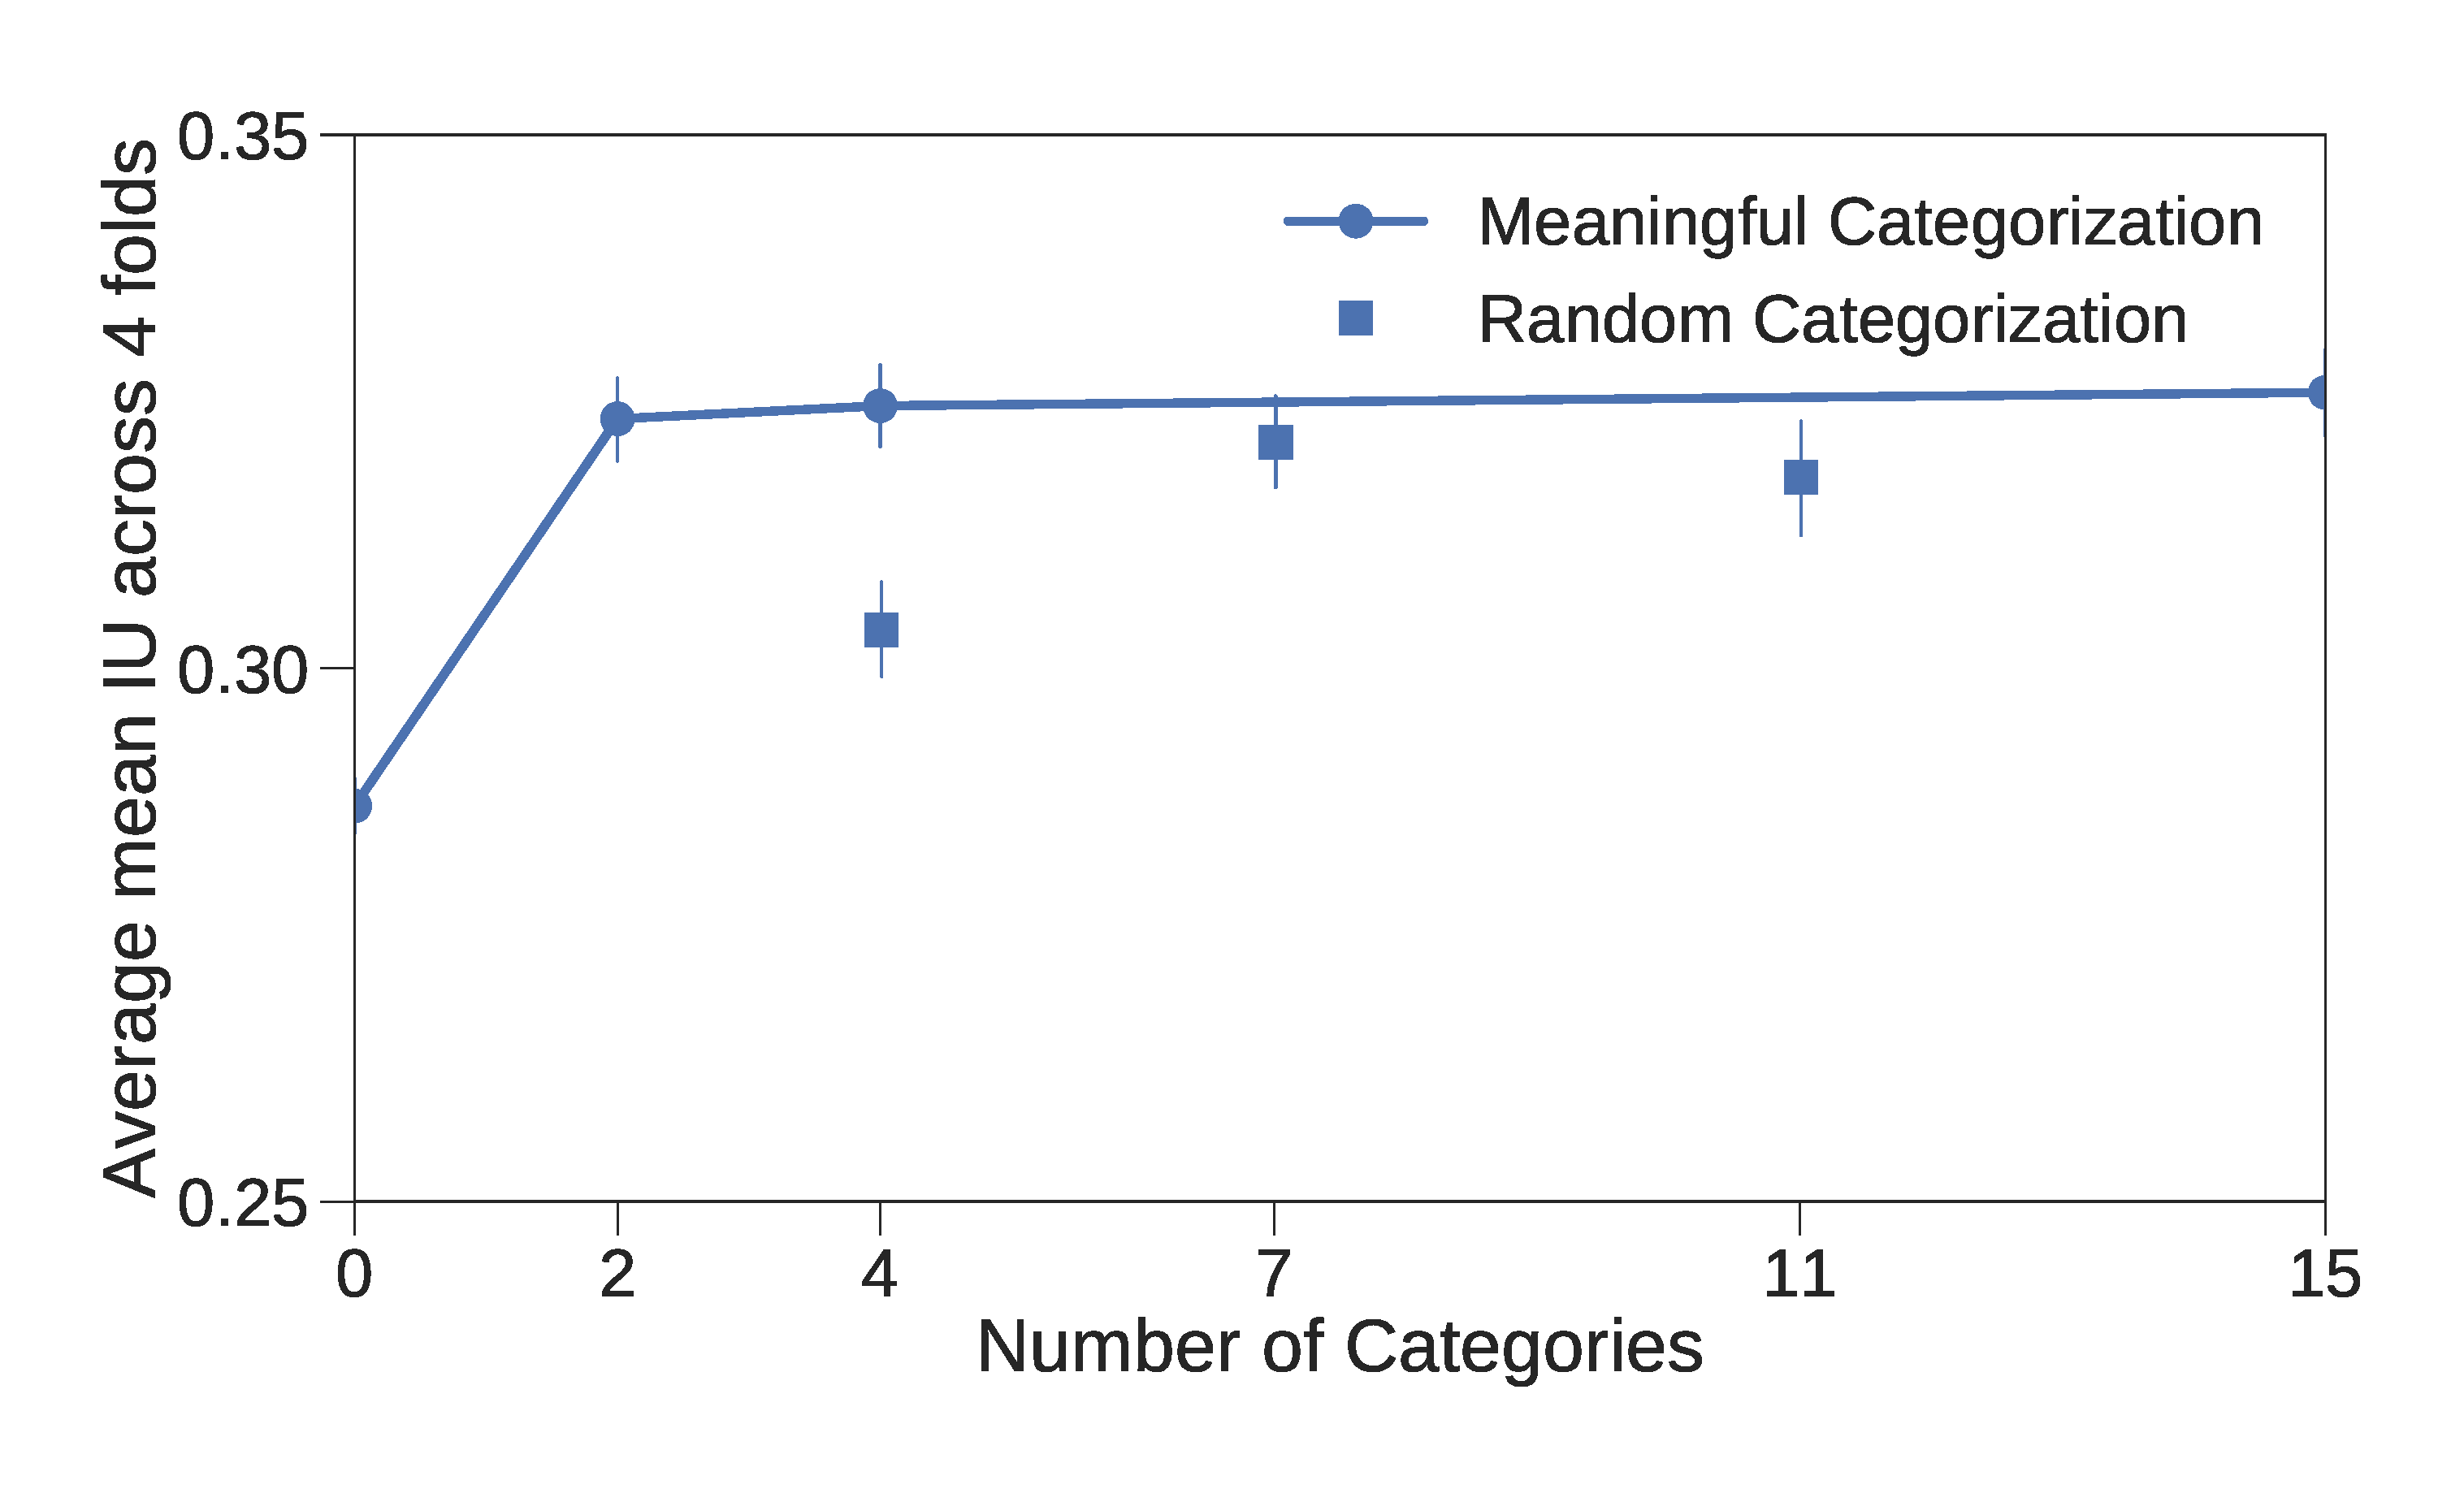
\includegraphics[width=1.\linewidth]{img/num_classes.eps}
\caption{
Test performance for models fine-tuned from pre-trained weights using data of categorized pre-training classes.
Isolated error bars denote random categorizations (RC) of the 15 classes, while error bars located on lines denote the meaningful categorization.
Zero categorize means no pre-trained weights used and the model was random initialized.
The displayed mean IU/mean accuracies and standard deviations were averaged over four folds listed in Table \ref{tab:robustness}.
The trend shows that binarizing and categorizing classes had little negative effect on feature transferability.
}
\label{fig:categories}
\end{figure}


%%%%%%%%%%%%%%%%%%%%%%%%%%%%%%%%%%%%%%%%%%%%%%%%%%%%%%%%%%%%
%%%%%%%%%% PU Learning
%%%%%%%%%%%%%%%%%%%%%%%%%%%%%%%%%%%%%%%%%%%%%%%%%%%%%%%%%%%%

\subsection{Learn to classify with positive and unlabeled samples}
\label{subsec:pulearning}


\paragraph{2-dimensional moons dataset}

Figure \ref{fig:moons} shows the decision boundaries of a 2-layer multilayer perceptron, with 6 neurons per layer, trained with the weighted loss, the sigmoidal loss and the bootstrapping loss.
Four hundred samples per class were drawn randomly from two interleaving half circles with noises added with a minor standard deviation.
The leftmost column in the figure shows the multilayer perceptron trained with complete positive labels and the normal logistic loss while the other three columns show the classifier trained with half of the positive examples labeled as negative.
For sigmoidal negative loss, the mislabeled positive examples faraway from the decision boundary have smaller derivatives the ones closer to but still distant from the decision boundary.
As a consequence, optimization performed as counting the weights update contributions differently for confident and unconfident prediction instead of simply decreasing the overall estimation for the negative loss.
The result decision boundary becomes more distant from the positive cluster, and confident predictions are made in more areas of the space.
% The positive examples push the decision boundary away from the positive cluster while negative examples closed to the decision boundary instead of those away from the decision boundary pull the decision boundary towards the positive cluster.

%%%%%%%% FIGURE MOONS

\begin{figure*}
\begin{center}
% \fbox{\rule{0pt}{2in} \rule{.9\linewidth}{0pt}}
   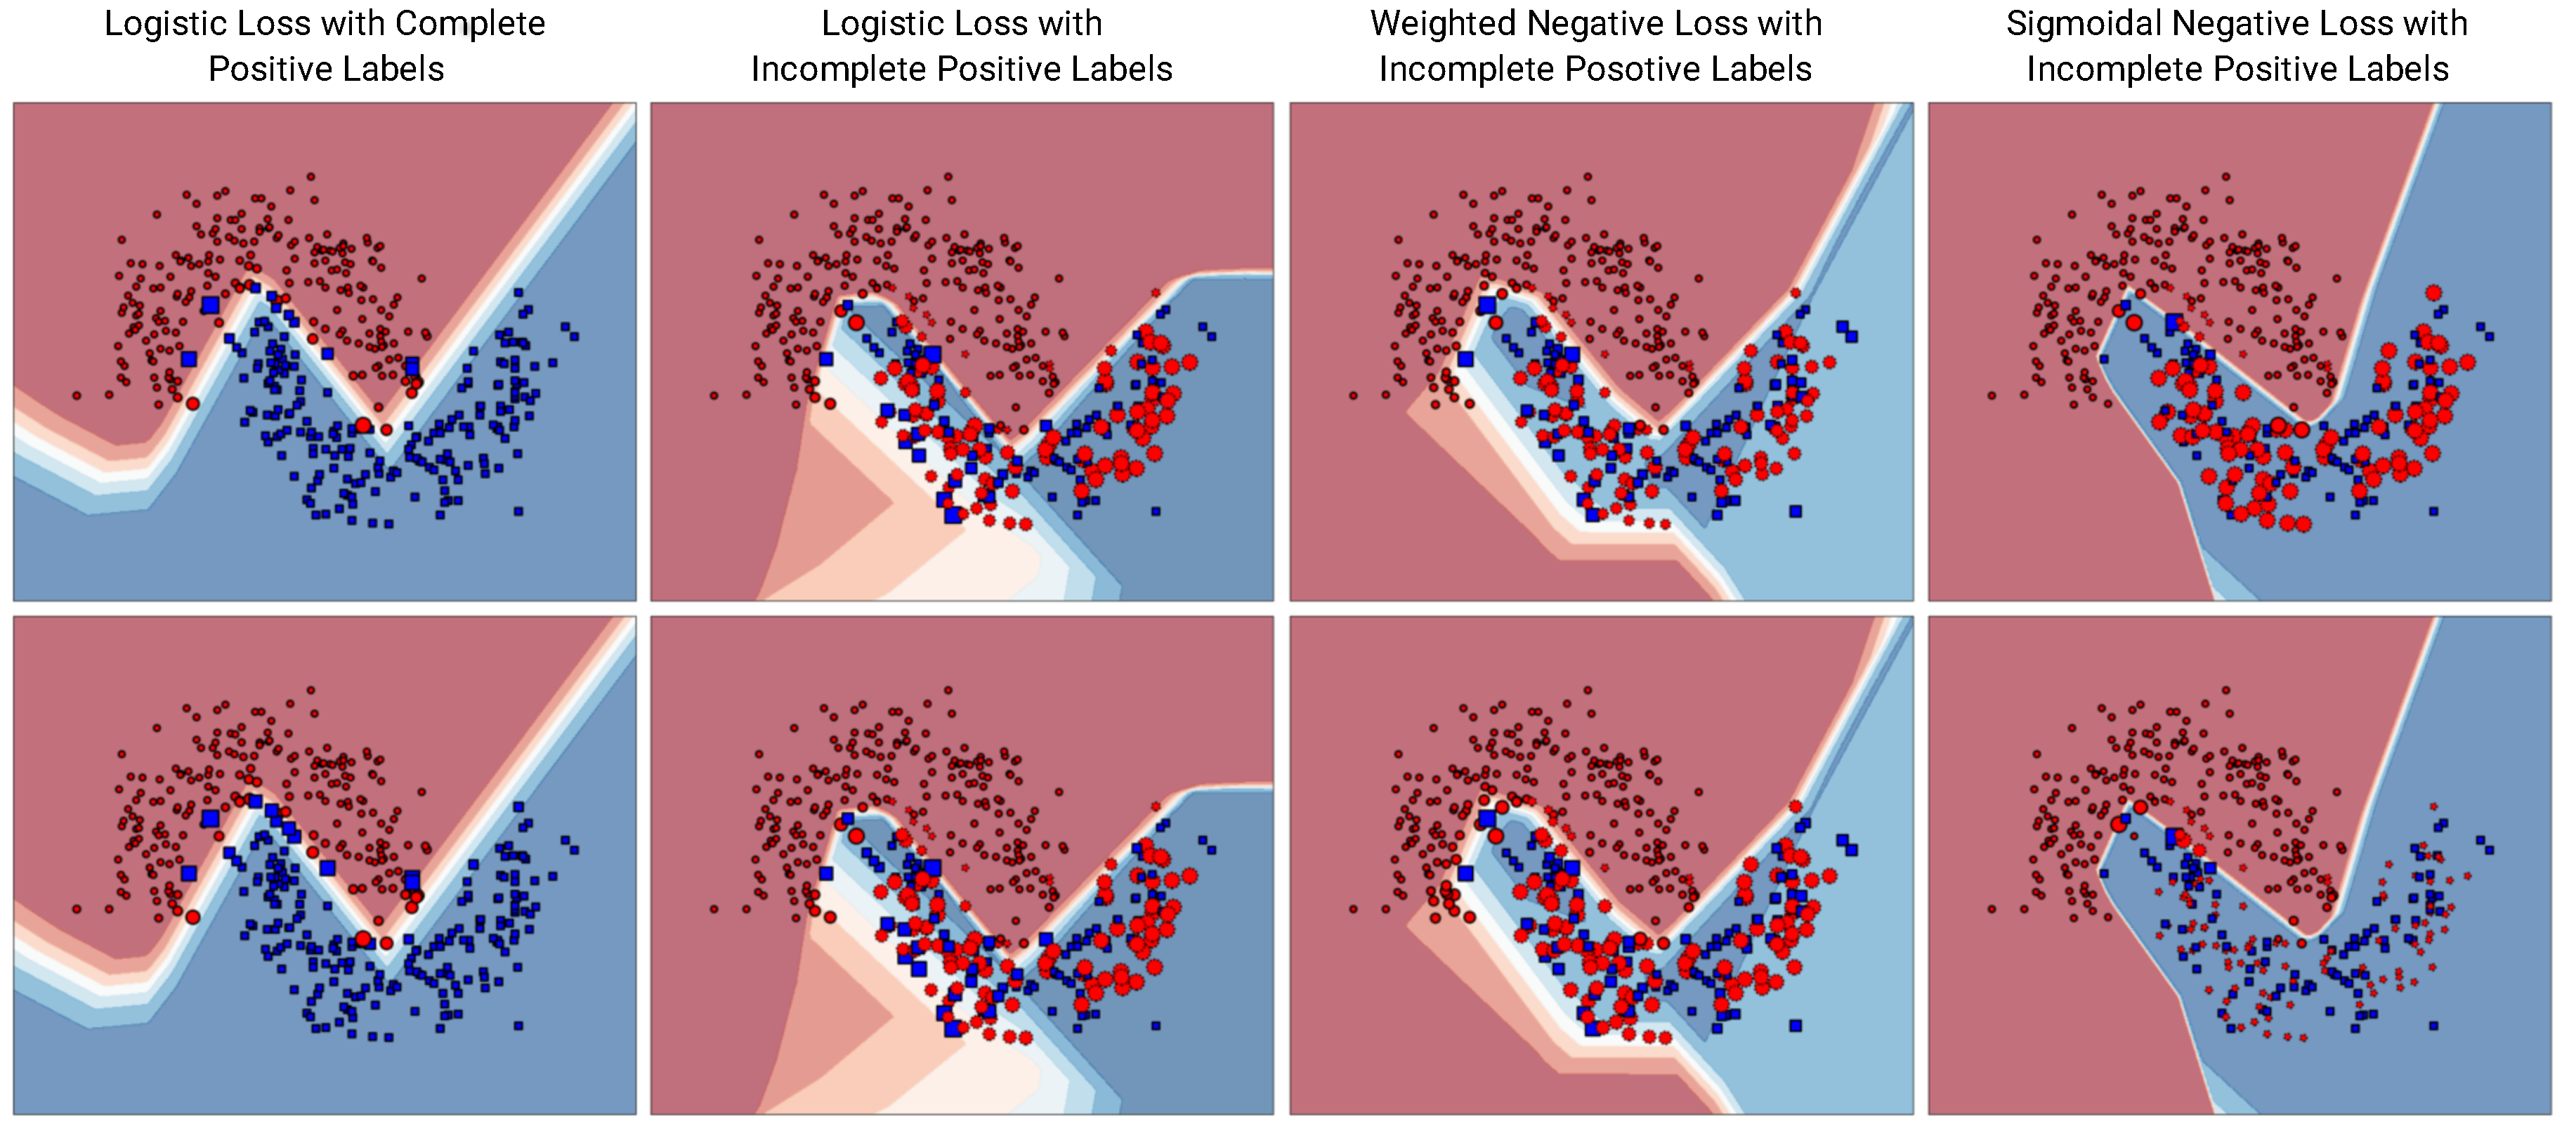
\includegraphics[width=0.95\linewidth]{img/moons}
\end{center}
   \caption{
   Decision boundaries, optimal losses, and derivatives of a 2-layer multilayer perceptron trained with different losses on a 2D moons dataset with the unlabeled positive.
   The \textbf{top row} demonstrates the per-class normalized training losses with \textbf{markers sizes} and the \textbf{bottom row} displays the per-class normalized loss derivatives w.r.t the output with marker sizes.
  %  The \textbf{leftmost} figures have complete positive labels, meaning the positive and negative labels are all correct, whereas, in \textbf{the other figures} only half of the positives were correctly labeled and the rest were mixed with the negative samples.
   A \textbf{red circle} indicates an example labeled as positive and a \textbf{blue square} indicates the example has a negative label.
   The \textbf{background colors} represent the probability for the area to be positive given by the classifier trained with the given samples and labels: \textbf{red} for high probability areas, \textbf{blue} for low probability areas and \textbf{white} for the class transition areas, i.e.decision boundaries.
   Compared to the normal logistic loss and weighted logistic loss, the decision boundary optimized with sigmoidal negative loss is more distant from the positive cluster.
   The sigmoidal negative loss has saturated losses and low derivatives for predictions farther from the decision boundary.
   }
\label{fig:moons}
\end{figure*}

\paragraph{CIFAR dataset}

Images from the CIFAR10 dataset were used as positive (P) examples, and images from the CIFAR100 dataset were considered as the negative (N) examples.
We trained a CNN model to classify images into eleven classes: ten positive classes from CIFAR10 and a negative class for images from CIFAR100.
To synthesize a PU learning setup, we correctly labeled only part of positive images from CIFAR10 and the rest were assigned negative labels together with CIFAR100 images, forming the unlabeled (U) set.
An eight layer CNN model was trained with different choices of losses and with the labeled positive examples and unlabeled examples.
Model performances were then evaluated on a separate test set of combined CIFAR10 and CIFAR100 with true labels.

The architecture of the CNN model can be found in Appendix \ref{sec:support}.
Each model was trained from scratch with Adam optimizer and base learning rate 0.0001.
Experiments were repeated three times with random split of P set, and U set and standard deviations were around 0.01 if not explicitly mentioned.
Note that there is no category overlap between CIFAR10 dataset and CIFAR100 dataset.

%%%%%%%% TABLE CIFAR10 50%

Table \ref{tab:cifar} summarizes the test precisions and recalls of using different losses to learn with true positive labels and noisy negative labels, compared to training with the normal cross-entropy loss.
With 50\% of the positive example correctly labeled and the rest assigned negative labels, the normal cross-entropy loss led to an imbalanced model with high precision but low recall, and therefore with a low f1-score.
By reweighing the negative loss by a factor of 0.5, we were able to balance precision and recall and improve the resulting f1-score significantly.
Sigmoidal negative loss and hard bootstrapping loss were able to achieve even slightly better f1-scores than the weighted negative loss, though not as good as training with clean labels with the same number of positive examples.
It is noteworthy that the weighted negative loss and hard bootstrapping loss achieved more balanced precision and recall than the sigmoidal negative loss.
That is because the two former losses were weighted by classes frequency of observed labels, around 0.67 for the negative class and 2 for positive classes, whereas the sigmoidal negative loss was not.
Reweighing the sigmoidal negative loss by observed label frequencies would trade too much precision for recall (0.74 and 0.83 respectively), resulting in a worse f1-score than not reweighing losses.
The sigmoidal negative loss seems to be easier over-balancing with the same choice of class weights.
% Besides, the optimal precision and recall for sigmoidal negative loss seem more unstable which may relate to the nonconvex class-dependent loss.


\begin{table}[t]
\resizebox{\columnwidth}{!}{
\centering
\begin{tabular}{ll|llll}
Annotation  & Loss & acc. & mean prec. & mean rec. & mean $F_1$ \\
\hline
P+N         & CrossEntropyU.   & 0.87 & 0.88 & 0.82 & 0.85 \\
50\%(P+N)   & CrossEntropyU.   & 0.83 & 0.84 & 0.78 & 0.80 \\
50\%P+U     & CrossEntropyU.   & 0.66 & 0.94 & 0.38 & 0.49 \\
\hline
50\%P+U     & WeightedNeg.     & 0.78 & 0.75 & 0.75 & 0.76 \\
50\%P+U     & SigmoidalNeg.    & \textbf{0.81} & \textbf{0.85$\pm0.03$} & 0.72$\pm0.03$ & 0.77 \\
50\%P+U     & BootstrapHard    & 0.80 & 0.76 & \textbf{0.81} & \textbf{0.78} \\
\end{tabular}
}
\caption{
Overall accuracy, the average of precision, recall, and f1-score over classes on a test set of the CIFAR dataset with true labels.
CIFAR10 images were used as positive images (P), and CIFAR100 images were used as negative images (N).
The top columns summarize the upper bound, lower bound and reference for learning with positive and unlabeled examples.
\textbf{Upper bound} Model trained with the complete positive and negative labels;
\textbf{Reference} Model trained with 50\% of the positive and negative examples;
\textbf{Lower bound} Model trained with 50\% labeled positive examples and unlabeled examples;
The proposed losses should achieve as high recall as possible while keeping the precision high as well.
The modified hard bootstrap loss achieved the highest average f1-score with 50\% positive examples unlabeled.
}
\label{tab:cifar}
\end{table}


%%%%%%%% FIGURE Varying positive annotating percetage

By varying the percentage of labeled positive examples, we compared learning with the labeled positive examples and noisy negative examples with the three different losses as shown in Figure \ref{fig:pct_annotating}.
Similarly as a result at 50\% positive examples labeled, the sigmoidal negative loss and hard bootstrapping loss had only little improvement compared to the weighted negative loss.
The assumption we made for the sigmoidal negative loss was that the probability of a negative example being wrong is dependent on the confidence.
However, the synthesized mislabeled positive examples were distributed at random when we synthesized them, meaning that the probability for a negative label being wrong is independent of the underlying distribution of the inputs.
No matter where the decision boundary is, such uniformly distributed incorrect negative labels are independent of the prediction confidence.
Therefore, it is expected for the sigmoidal negative loss and bootstrapping loss to have similar performance as the weighted negative loss.

Figure \ref{fig:pct_annotating} also demonstrates that learning with a subset of reliable negative examples (PN setup) outperformed learning with positive and unlabeled examples (PU setup) for any percentage of labeled positives and any losses being used.
This result was expected because the PN setup delivers extra information about which images in the unlabeled set are negative.
The PU setup is therefore only relevant when it is impossible to easily construct a subset of negative examples from the unlabeled data.
Otherwise, training with true positive and negative labels, and potentially with semi-supervised learning, would be superior to training with positive and unlabeled examples only.

\begin{figure}[t]
\centering
   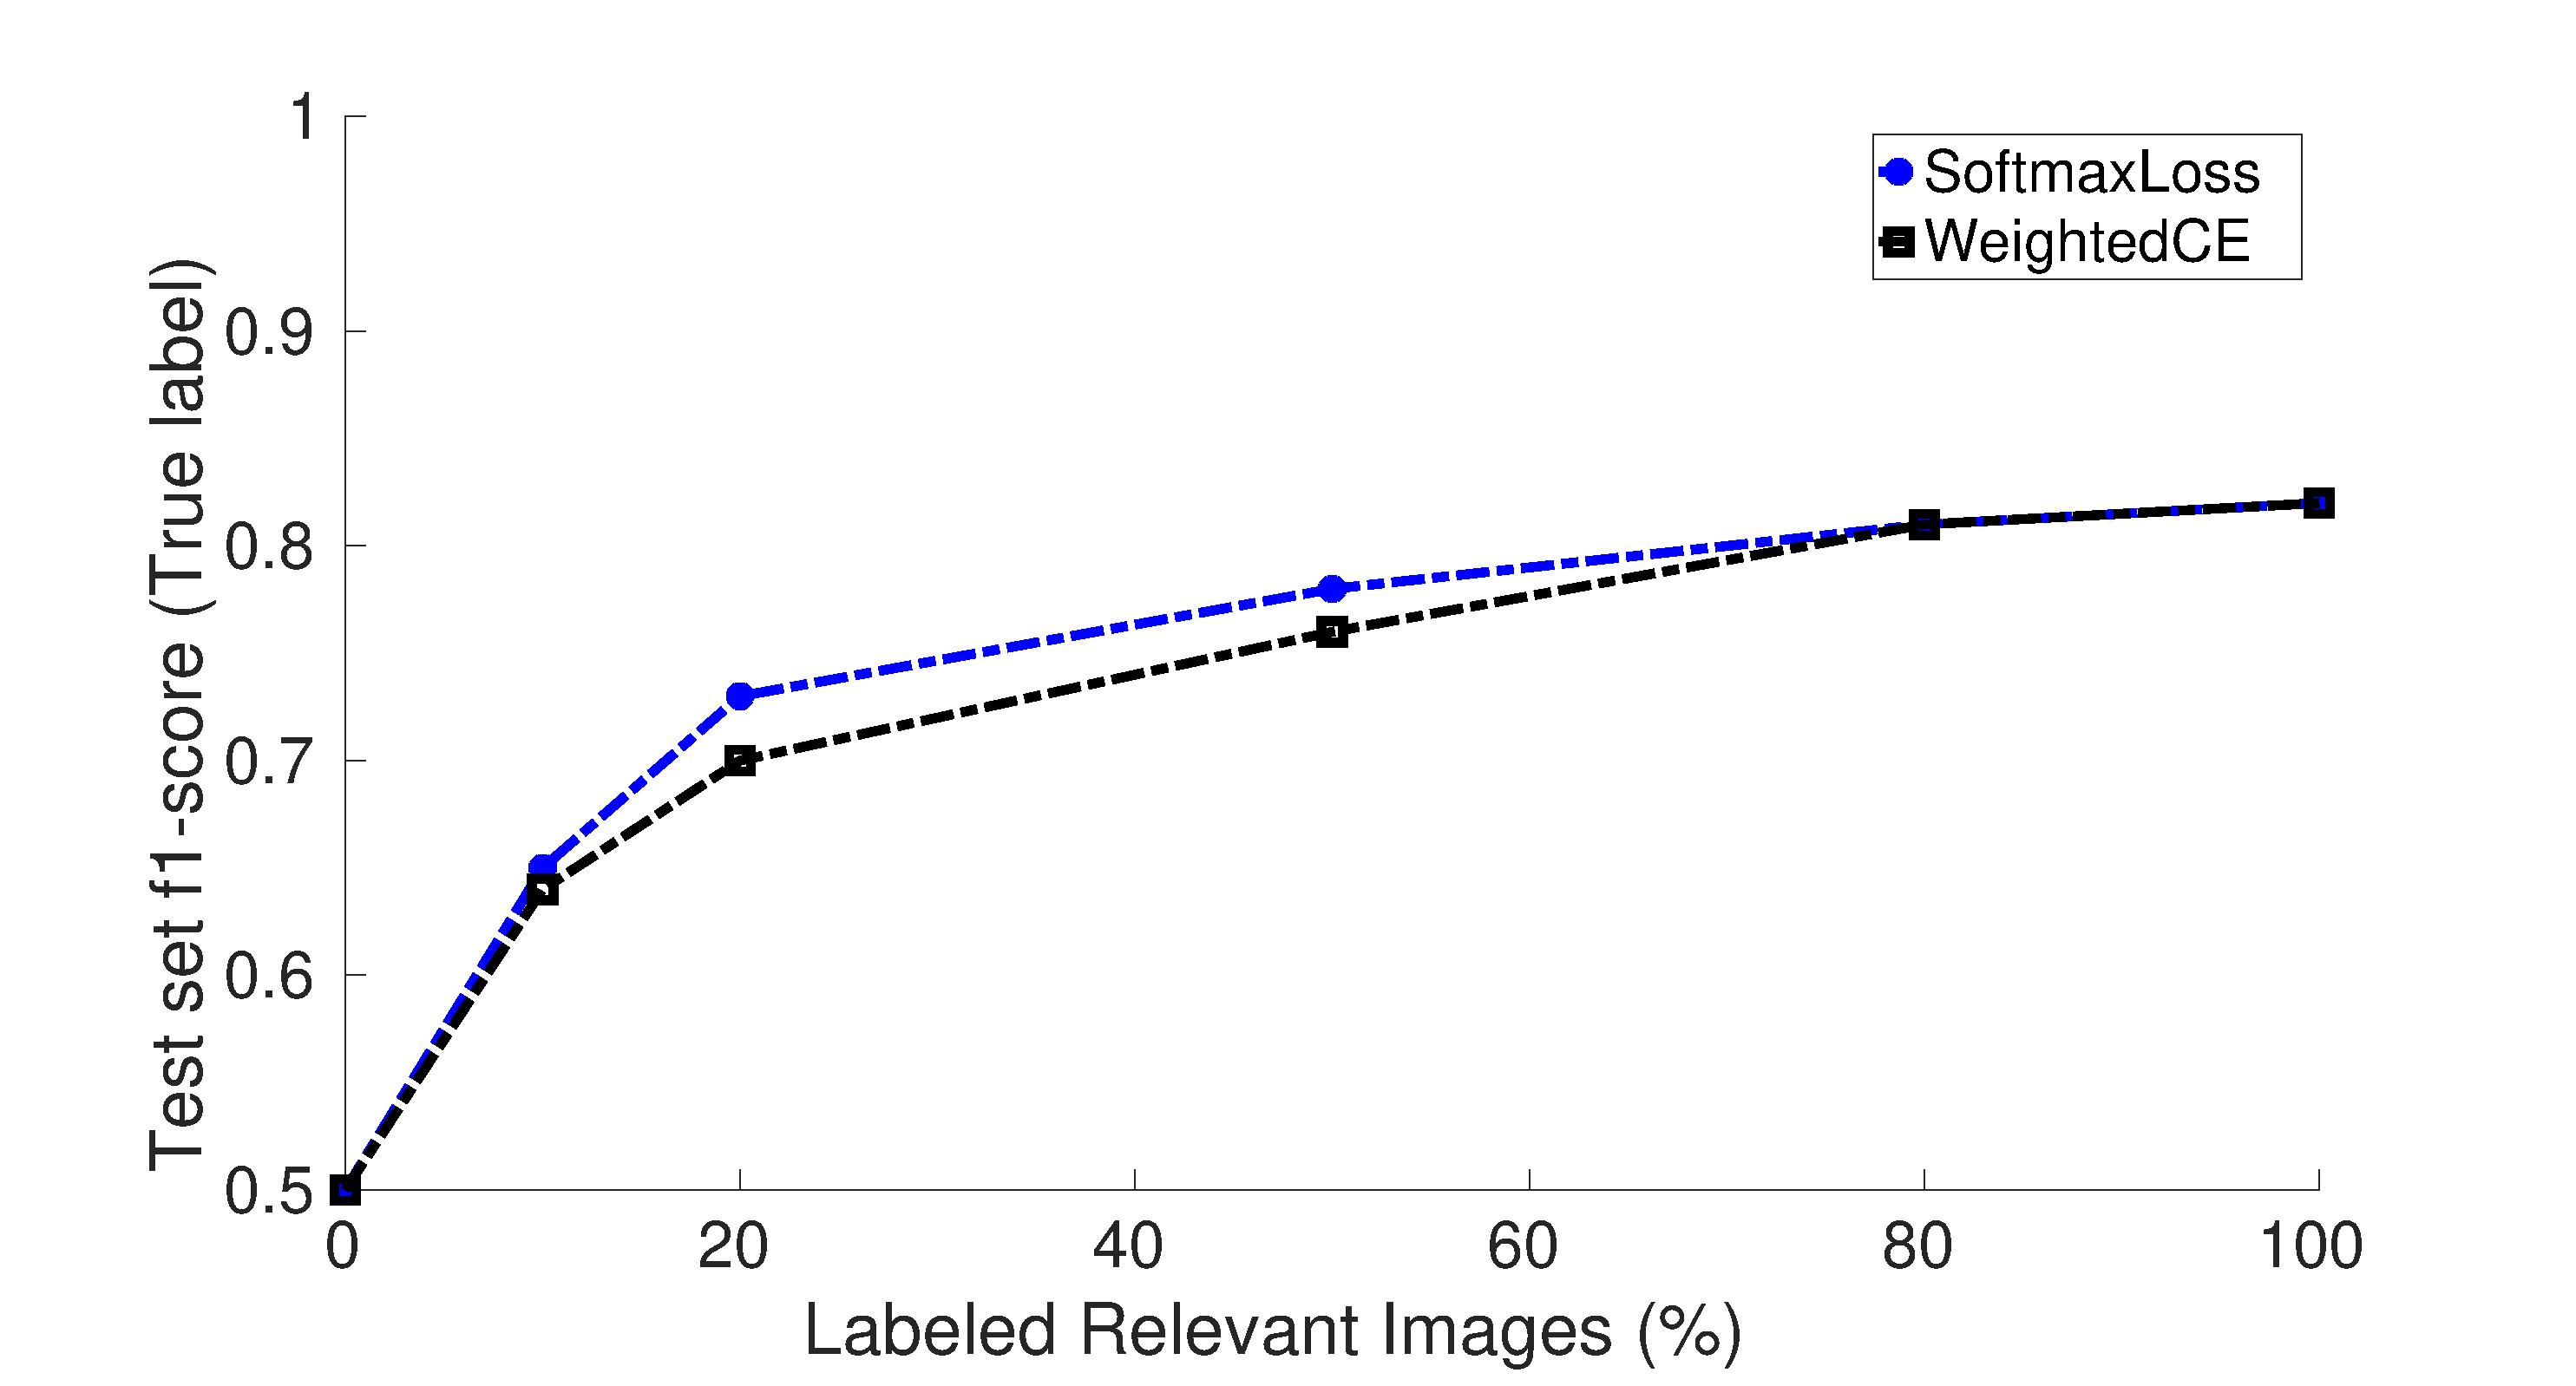
\includegraphics[width=1.05\linewidth]{img/pu_vs_pn}
\caption{
Comparing the f1-score achieved for weighted negative loss, sigmoidal loss and hard bootstrapping loss with varying percentage of labeled positive images
\textbf{P+N} represents training with the percentage of images with reliable positive and negative labels, and \textbf{P+U} stands for training with the positive (P) and unlabeled (U) sets.
The test performances of the three different losses did not show significant difference with the labeled positive percentage varying from 0\% to 100\%.
}
\label{fig:pct_annotating}
\end{figure}

%%%%%%%% Text Segmentation Pascal VOC2011
\paragraph{Pascal VOC2011 segmentation task}

To study the effect of sigmoidal negative loss on compensating incomplete segmentations, we used again the PASCAL VOC2011 dataset with extra segmentation \cite{hariharan2011semantic}.
We synthesized inexhaustive segmentations the same way as described in Section \ref{subsec:robustness}.
The same AlexNet-FCN model was trained together with the different loss functions for class 0 to predict binary segmentation, determining whether a pixel belongs to an object or not.
Only single-object images were used for training and testing to avoid the influence of two adjacent objects joining as one object because of binary segmentation.
The same hyperparameters for optimization were used as in Section \ref{subsec:robustness}.
The trained models were evaluated with the test set of PASCAL VOC2011 segmentation dataset with binary segmentations.

As shown in Table \ref{tab:pusegment}, the sigmoidal negative loss achieved the highest mean accuracy, approximately 0.07 better than training with the normal cross entropy loss.
In contrast to the improvement of mean accuracy, mean IU for models trained with either weighted negative loss or sigmoidal negative loss did not show significant improvement compared to the normal cross entropy loss.
The increase in the mean accuracy was caused by an increase in
foreground accuracy and a decrease in background accuracy.
In other words, the sigmoidal loss balances precision for recall, similarly as observed in training the CIFAR dataset.
The decrease in precision, however, can interfere the improvement mean IU since the mean IU counts for both low false positive rate and low false negative rate.

%%%%%%%% Text Fine-tuning performance with exponential loss

We then applied the sigmoidal negative loss to the pre-training phase of the experiment for inexhaustive segmentations in Section \ref{subsec:robustness}.
We were able to recover the negative influence of inexhaustive segmentations on the fine-tuning performance of the pre-trained models.
Note that we learned foreground/background segmentation instead of multi-class segmentation when applied the sigmoidal negative loss because we discovered binarizing pre-training classes had little effect to feature transferability in this experimental setup.
% {TODO} and the potential difficulty in extending sigmoidal negative loss to a multi-class scenario as we will discuss more in Section \ref{sec:discussion}.


%%%%%%%% TABLE Segmentation Pascal VOC2011
\begin{table}[t]
\resizebox{\columnwidth}{!}{
\centering
\begin{tabular}{ll|llll}
Annotation  & Loss & overall acc. & mean acc. & f.w. IU & mean IU \\
\hline
% Complete            & CrossEnt.U       &  0.88 & 0.60 & 0.48 & 0.80 \\
% 50\%Unsegmented     & CrossEnt.U       &  0.83 & 0.31 & 0.27 & 0.70 \\
% 50\%Unsegmented     & WeightedU        &  0.83 & 0.34 & 0.29 & 0.70 \\
% 50\%Unsegmented     & ExponentialU     &  0.83 & 0.34 & 0.29 & 0.70 \\
Complete       & CrossEntropy       &  0.90 & 0.85 & 0.82 & 0.75 \\
50\%Unseg.     & CrossEntropy       &  0.85 & 0.68 & 0.73 & 0.60 \\
50\%Unseg.     & WeightedNeg.       &  0.84 & 0.71 & 0.73 & \textbf{0.62} \\
50\%Unseg.     & SigmoidalNeg.      &  0.83 & \textbf{0.75} & 0.72 & \textbf{0.62} \\
\end{tabular}
}
\caption{
The best foreground/background segmentation performance achieved on the test set of PASCAL VOC2011 segmentation dataset with the normal cross entropy loss, weighted negative loss, and sigmoidal negative loss in the presence of inexhaustive segmentation.
A class weight of 0.7:1.75 was used to balance the sample frequency differences of the two classes.
The negative loss was further weighted by a factor of 0.5 for the weighted negative loss.
Mean accuracy is equivalent to the average recall over the two classes.
Mean IU is the average intersection over union ratio (IU) over two classes and f.w. IU is the frequency weighted average of IU over the two classes.
Experiments were repeated twice and standard deviations were approximately 0.02.
The sigmoidal negative loss achieved a better mean accuracy than weighted negative loss and a similar mean IU as the weighted negative loss.
Both losses performed better than the normal cross entropy loss in the presence of 50\% objects unsegmented.
}
\label{tab:pusegment}
\end{table}


%%%%%%%% Figure Segmentation Pascal VOC2011
Selective predictions made by models trained with the sigmoidal negative loss and the cross entropy loss were presented in Figure \ref{fig:pusegment}.
For these two example images, the model trained with the cross entropy loss failed to segment objects from images whereas sigmoidal negative loss predicted segmentations on the position of the objects.
The coarse outlines were mainly due to the limited compacity of the FCN-AlexNet model.
The third column shows predictions given by model trained with complete training segmentation, and it did not produce more accurate outlines.

\begin{figure}
\centering
  \begin{minipage}{\columnwidth}\footnotesize
  \centering
  \subsubfloat{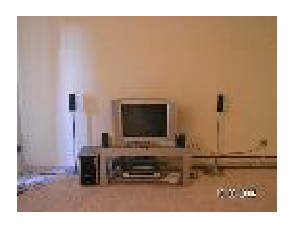
\includegraphics[width=0.19\columnwidth]{img/2007_002132}}{Raw}
  \subsubfloat{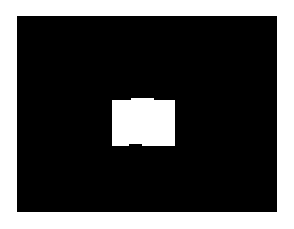
\includegraphics[width=0.19\columnwidth]{img/2007_002132_label}}{Label}
  \subsubfloat{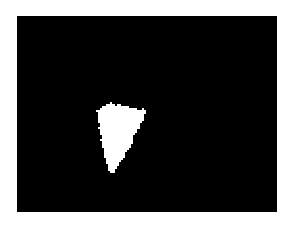
\includegraphics[width=0.19\columnwidth]{img/2007_002132_up_pred}}{Complete}
  \subsubfloat{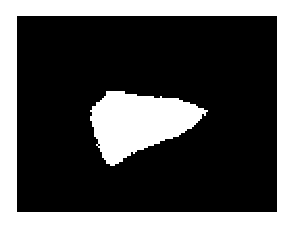
\includegraphics[width=0.19\columnwidth]{img/2007_002132_exp_pred}}{ExpU.}
  \subsubfloat{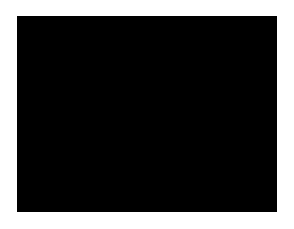
\includegraphics[width=0.19\columnwidth]{img/2007_002132_low_pred}}{CrossEnt.}
  \subsubfloat{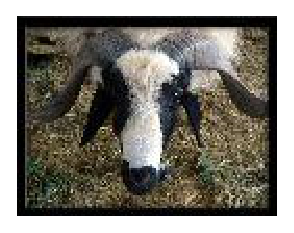
\includegraphics[width=0.19\columnwidth]{img/2007_002618}}{Raw}%
  \subsubfloat{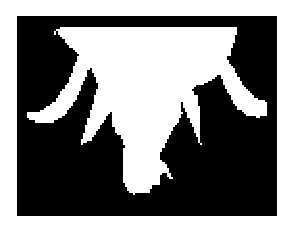
\includegraphics[width=0.19\columnwidth]{img/2007_002618_label}}{Label}
  \subsubfloat{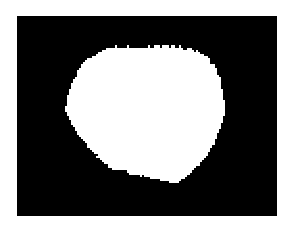
\includegraphics[width=0.19\columnwidth]{img/2007_002618_up_pred}}{Complete}
  \subsubfloat{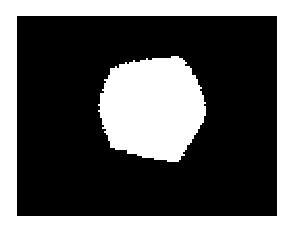
\includegraphics[width=0.19\columnwidth]{img/2007_002618_exp_pred}}{ExpU.}
  \subsubfloat{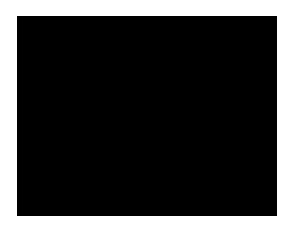
\includegraphics[width=0.19\columnwidth]{img/2007_002618_low_pred}}{CrossEnt.}
  \end{minipage}
\caption{
Selective predictions made by models trained with the sigmoidal negative loss and the cross-entropy loss.
This figure presented two selective images for which the model trained with the cross entropy loss failed to segment objects, and the one with sigmoidal negative loss succeed.
}
\label{fig:pusegment}
\end{figure}
